\documentclass[letterpaper,11pt]{article}
\usepackage{jheppub}
\usepackage{tikz}

\usetikzlibrary{decorations.pathreplacing}
\usetikzlibrary{shapes.misc, positioning}



\definecolor{iocolor}{RGB}{169,205,236}
\definecolor{hlvcolor}{RGB}{224,235,245}
\definecolor{hscolor}{RGB}{166,166,166}
\definecolor{layercolor}{RGB}{218,218,218}
\definecolor{featcolor}{RGB}{202,203,229}
\definecolor{grucolor}{RGB}{222, 236, 239}

%\definecolor{hlvlinecolor}{RGB}{12, 178, 236}
%\definecolor{featurelinecolor}{RGB}{100, 159, 206}
\definecolor{hlvlinecolor}{RGB}{0, 148, 197}
\definecolor{featurelinecolor}{RGB}{0, 43, 152}
\definecolor{hslinecolor}{RGB}{85, 85, 85}



\begin{document}

%%%%%%%%%%%%%%%%%%%%%%
\section*{Anomalous Jet Identification via Variational Recurrent Neural Network}
Authors: Alan Kahn, Julia Gonski, In\^{e}s Ochoa, Daniel Williams, Gustaaf Brooijmans \\ \textit{Nevis Laboratories, Columbia University, Address}\\

%\noindent \textit{Please do not write an introduction to anomaly detection - we will have one introduction at the beginning.  Furthermore, please give your method a concise name - it is fine to say \textbf{Concise Name: Longer Name that is More Specific.}  The length limit is five pages of text (not included references), with fewer pages preferred, and at most one additional page of figures if needed.}

\subsection{Method}
\label{sec:method}

Our method employs a Variational Recurrent Neural Network (VRNN) to model jets as a sequence of constituents. A VRNN is a sequence-modeling architecture which replaces the standard encoder-decoder architecture of a Recurrent Neural Network with a Variational Autoencoder. This allows the VRNN to perform both sequence modeling as well as \textit{Variational Inference}, which has been shown to be a very powerful tool in the task of Anomaly Detection [Ref]. Figure \ref{fig:VRNN} shows a diagram of one VRNN cell. The VAE portion of the architecture is displayed on the top row of layers in the diagram, where an input constitent's four-momentum components are input as a vector $x(t)$, which is encoded into a gaussian distribution in the latent space $z$, and then decoded to produce a reconstruction of the same input constituent's components $y(t)$. The variable $t$ refers to the \textit{time-step}, which advances as the sequence is processed, and can be interpreted as the constituent number currently being processed by the model. 

Inputs to the VRNN consist of sequences of jet 4-vector constituent components $p_{T}$, $\eta$, and $\phi$, where we assume massless constituents. Before training, we apply a pre-processing method which boosts each jet to the same reference mass, energy, and orientation in $\eta-\phi$ space, such that all jets are superficially the same with the only differences being their substructure. In addition, our pre-processing method includes a choice of \textit{sequence ordering}, in which the constituent sequence input into the model is sorted by $k_{t}$-distance instead of by constituent $p_{T}$. In more detail, the $n^{th}$ constituent in the list, $c_{n}$, is determined to be the constituent with the highest $k_{t}$-distance relative to the previous constituent, with the first constituent in the list being the highest $p_{T}$ constituent. This ordering is chosen such that non QCD-like substructure, characterized by two or more separate cores of constituent clusters within in the jet, is more easily characterized by the sequence. When compared to $p_{T}$-sorted constituent ordering, our sequence consistently travels between each cluster, making their existence readily apparent and easy to model. As a result, we have observed a significant boost in performance due to this choice.
\begin{align*}
c_{n} &= max(p_{Tn}\Delta R_{n, n-1})
\end{align*}
The loss function used is very similar to that of an ordinary Variational Autoencoder. It consists of a mean-squared-error (MSE) loss between input constituents and generated output constituents as a reconstruction loss, as well as a weighted KL-Divergence from the latent space prior to the learned approximate posterior distribution. Since softer constituents contribute less to the overall classification of jet substructure, each KL-Divergence term, computed constituent-wise, is weighted by the constituent's $p_{T}$-fraction with respect to the jet's total $p_{T}$, averaged over all jets in the dataset to avoid correlations with constituent multiplicity. An additional weight coefficient is enforced as a hyperparameter, and has been optimized to be 0.1 in our studies. 
\begin{align*}
\mathcal{L}(t)=MSE+0.1\overline{p_T}(t)D_{KL}
\end{align*}
The architecture is built with 16 dimensional hidden layers, including the hidden state, with a two-dimensional latent space. All hyperparameters used result from a hyperparameter optimization scan. 

Our model is trained on the leading and sub-leading jets of each event, where our input datasets consist of the entirety Background and Black Box events. After training, we evaluate each jet in the dataset and assign it an \textit{Anomaly Score}, defined as follows, where $D_{KL}$ is the KL-Divergence between the encoded posterior distribution and learned prior distribution:
\begin{align*}
\text{Anomaly Score} &= 1 - e^{-\overline{D_{KL}}}
\end{align*}


Since the LHC Olympics challenge entails searching for a signal on the event-level instead of the jet-level, we determine an overall \textit{Event Score} by choosing the most anomalous score between the leading and sub-leading jets. To ensure consistency between training scenarios, Event Scores are subject to a transformation in which the mean of the resulting distribution is set to a value of 0.5, and Event Scores closer to 1 correspond to more anomalous events. 

%please introduce the motivation for your method (not anomaly detection in general), how it works, and how you have implemented it. Please include details about how you trained your algorithms and how your picked your hyperparameters.


%VRNN Diagram
\begin{figure}
  \begin{center}
  
    \def\layersep{2.5cm}
    
    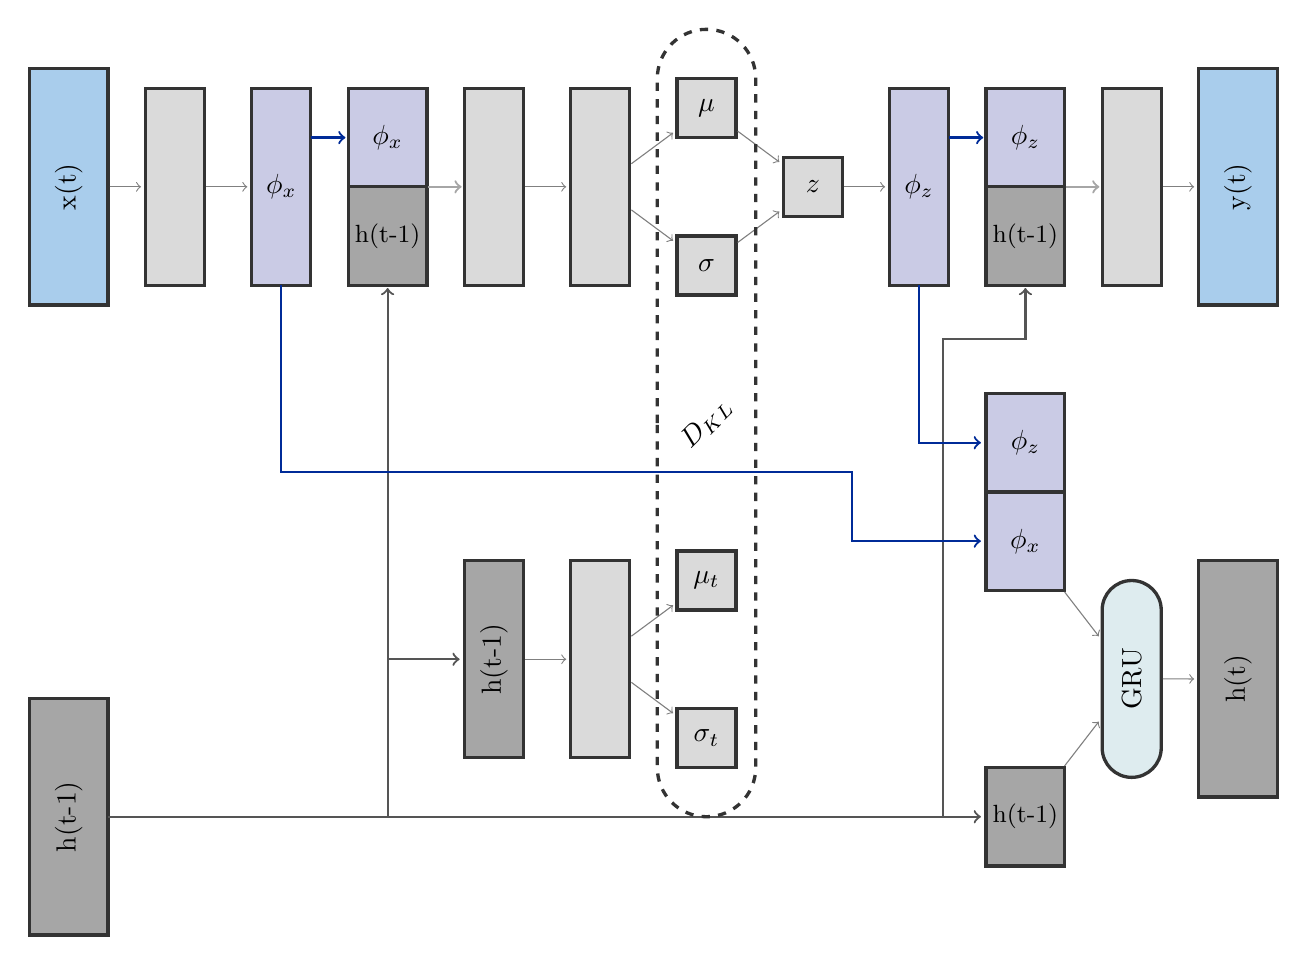
\begin{tikzpicture}[shorten >=1pt,->,draw=black!50, node distance=\layersep]
        \tikzstyle{every pin edge}=[<-,shorten <=1pt]
        \tikzstyle{neuron}=[rectangle,fill=black!25, draw=black!80, very thick, minimum width=0.75cm, minimum height=2.5cm, inner sep=0pt]
        \tikzstyle{input neuron}=[neuron, fill=iocolor, rotate=90, minimum width = 3cm, minimum height = 1cm];
        \tikzstyle{gru}=[rounded rectangle, draw=black!80, very thick, rotate=90, minimum width = 2.5cm, minimum height = 0.75cm, inner sep=0pt];
        \tikzstyle{output neuron}=[neuron, fill=red!50];
        \tikzstyle{latent neuron musig}=[neuron, fill=black!10!yellow];
        \tikzstyle{latent neuron}=[neuron, fill=layercolor, minimum height=0.75cm, minimum width=0.75cm];
        \tikzstyle{layer neuron}=[neuron, fill=layercolor];
        \tikzstyle{hidden neuron}=[neuron, fill=hscolor];
        \tikzstyle{feature neuron}=[neuron, fill=featcolor];
        \tikzstyle{hlv neuron}=[neuron, fill=hlvcolor];
        \tikzstyle{annot} = [text width=4em, text centered]
        \tikzstyle{kldash} = [rounded rectangle, draw=black!80, dashed, very thick, minimum width=1cm, minimum height=10cm, inner sep=0pt];
    
        % Draw the input layer nodes
        %\foreach \name / \y in {1,...,6}
        % This is the same as writing \foreach \name / \y in {1/1,2/2,3/3,4/4}
        %    \node[input neuron] (I-\name) at (0,-\y) {};


        %INPUTS
        \node[input neuron] (Ix) at (0, -1) {x(t)};
        %\node[input neuron, fill=hlvcolor] (Ihlv) at (0, -5) {HLV};
        \node[input neuron, fill=hscolor] (Ihs) at (0, -9) {h(t-1)};
        \node[input neuron] (Oy) at (14.85, -1) {y(t)};
        \node[input neuron, fill=hscolor] (Ohs) at (14.85, -7.25) {h(t)};

        %Intermediate Layers
        \node[layer neuron] (h1) at (1.35, -1) {};
        \node[feature neuron] (phix) at (2.7, -1) {$\phi_{x}$};
        \node[feature neuron] (phiz) at (10.8, -1) {$\phi_{z}$};

        %Concatenated Layers
        \node[feature neuron, minimum width=1cm, minimum height=1.25cm] (catphixi) at (4.05, -0.375) {$\phi_{x}$};
        %\node[hlv neuron, minimum width=1cm, minimum height=1.25cm] (cathlvi) at (4.05, -1) {\small HLV};
        \node[hidden neuron, minimum width=1cm, minimum height=1.25cm] (cathsi) at (4.05, -1.625) {\small h(t-1)};

        \node[feature neuron, minimum width=1cm, minimum height=1.25cm] (catphizo) at (12.15, -0.375) {$\phi_{z}$};
        %\node[hlv neuron, minimum width=1cm, minimum height=1.25cm] (cathlvo) at (12.15, -1) {\small HLV};
        \node[hidden neuron, minimum width=1cm, minimum height=1.25cm] (cathso) at (12.15, -1.625) {\small h(t-1)};

        \node[feature neuron, minimum width=1cm, minimum height=1.25cm] (catphizh) at (12.15, -4.25) {$\phi_{z}$};
        \node[feature neuron, minimum width=1cm, minimum height=1.25cm] (catphixh) at (12.15, -5.5) {$\phi_{x}$};
        %\node[hlv neuron, minimum width=1cm, minimum height=1.25cm] (cathlvh) at (12.15, -6.75) {\small HLV};
        \node[hidden neuron, minimum width=1cm, minimum height=1.25cm] (cathsh) at (12.15, -9) {\small h(t-1)};
        

        %Intermediate Layers
        \node[layer neuron] (h2) at (5.4, -1) {};
        \node[layer neuron] (h3) at (6.75, -1) {};
        \node[layer neuron, fill=hscolor, rotate=90, minimum width=2.5cm, minimum height=0.75cm] (hs1) at (5.4, -7) {h(t-1)};
        \node[layer neuron] (hs2) at (6.75, -7) {};
        \node[layer neuron] (h4) at (13.5, -1) {};
        
        %Latent layers
        \node[latent neuron] (lmuz) at (8.1, 0) {$\mu$};
        \node[latent neuron] (lsiz) at (8.1, -2) {$\sigma$};
        \node[latent neuron] (lmuh) at (8.1, -6) {$\mu_{t}$};
        \node[latent neuron] (lsih) at (8.1, -8) {$\sigma_{t}$};
        \node[latent neuron] (lz) at (9.45, -1) {$z$};


        %GRU
        \node[gru, fill=grucolor] (gru) at (13.5, -7.25) {GRU};
  




        %Arrows
        %Hidden Layers
        \path (Ix) edge (h1);
        \path (h1) edge (phix);
        \path (h2) edge (h3);
        \path (hs1) edge (hs2);
        \path (lz) edge (phiz);
        \path (h4) edge (Oy);
        \path (gru) edge (Ohs);
        %\path (cathlvi) edge (h2);
        %\path (cathlvo) edge (h4);
        \path (catphixh) edge (gru);
        \path (cathsh) edge (gru);
      


        %Latent Space
        \path (h3) edge (lmuz);
        \path (h3) edge (lsiz);
        \path (hs2) edge (lmuh);
        \path (hs2) edge (lsih);
        \path (lmuz) edge (lz);
        \path (lsiz) edge (lz);

        

        %Other
        %\path (phix) edge (catphixi);
        %\path (phiz) edge (catphizo);



        %HLV Lines
        %\draw[->, draw=hlvlinecolor, thick] (0.5, -5) -- (3.3, -5) -- (3.3, -1) -- (3.55, -1);
        %\draw[->, draw=hlvlinecolor, thick] (3.2, -5) -- (11.4, -5) -- (11.4, -1) -- (11.65, -1);
        %\draw[->, draw=hlvlinecolor, thick] (11.4, -5) -- (11.4, -6.75) -- (11.65, -6.75);


        %Hidden State Lines
        \draw[->, draw=hslinecolor, thick] (0.5, -9) -- (4.05, -9) -- (4.05, -2.25);
        \draw[->, draw=hslinecolor, thick] (4.05, -7) -- (5.0, -7);
        \draw[->, draw=hslinecolor, thick] (4.05, -9) -- (11.62, -9);               
        \draw[->, draw=hslinecolor, thick] (11.1, -9) -- (11.1, -2.9375) -- (12.15, -2.9375) -- (12.15, -2.25);



        %phix,z lines
        
		\draw[->, draw=hscolor, thick] (4.56, -1) -- (5.025, -1);       
		\draw[->, draw=hscolor, thick] (12.66, -1) -- (13.125, -1);   
        
        \draw[->, draw=featurelinecolor, thick] (2.7, -2.25) -- (2.7, -4.625) -- (9.95, -4.625) -- (9.95, -5.5) -- (11.62, -5.5);
        \draw[->, draw=featurelinecolor, thick] (3.075, -0.375) -- (3.55, -0.375);

        \draw[->, draw=featurelinecolor, thick] (11.175, -0.375) -- (11.65, -0.375);
        \draw[->, draw=featurelinecolor, thick] (10.8, -2.25) -- (10.8, -4.25) -- (11.62, -4.25);
    
  



        %KL dashed box
        \node[gru, minimum width=10cm, minimum height=1.25cm, dashed] (kld) at (8.1, -4) {\rotatebox{-45}{$D_{KL}$}};

    \end{tikzpicture}
  
  \end{center}
  \caption{A Variational Recurrent Neural Network cell. The $x(t)$ and $y(t)$ layers represent respectively the input constituent and reconstructed constituents' four-momentum components $p_{T}$, $\eta$, and $\phi$. The $phi_{x}$ and $phi_{z}$ layers are \textit{feature-extracting layers} which encode a representation of the features in the input layer $x(t)$ and latent space $z$ respectively. $h(t-1)$ represents the current time-step's hidden state, which is updated each iteration via a transition function between $h(t-1$, $phi_{x}$, and $phi_{z}$ carried out by a Gated Recurrent Unit (GRU). At each timestep, the prior distribution defined by $\mu_{t}$ and $\sigma_{t}$ is determined from the current hidden state}
  \label{fig:VRNN}
\end{figure}

\subsection{Results on LHC Olympics}
\label{sec:results}

%\noindent \textit{We welcome results on any of the black boxes (BBs) as well as the R\&D dataset.  Please try to minimize any discussion of non-LHCO results.  Figures should be referenced like this: Fig.~\ref{fig:fig1}.}

We first present results with the R\&D dataset. In this study we want to directly investigate the performance of the Anomaly Score, and therefore refrain from imposing cuts on additional variables. Using the Event Score as a discriminator, we aim to reconstruc the $Z'$ mass peak within a contaminated dataset consisting of 895113 background events and 4498 signal events corresponding to a contamination level of 0.5\%,. Figure \ref{fig:m_v_s} shows the two-dimensional histogram of dijet mass vs Event Score, where we see the $Z'$ mass at 3500 GeV clearly visible at higher values of the Event Score. Figure \ref{fig:m_JJ} shows the one-dimensional dijet mass distributions before and after a cut on the Event Score at a value of 0.65, which is chosen to retain enough statistics in the background to display its smoothly falling behavior. We also plot the local significance of the signal, which we have computed for each bin. We see that a cut on the Event Score dramatically increases the significance of the excess from $1\sigma$ to $6\sigma$ at a signal contamination of 0.5\% while still retaining the smoothly falling behavior of the background

\begin{figure}[h!]
\centering
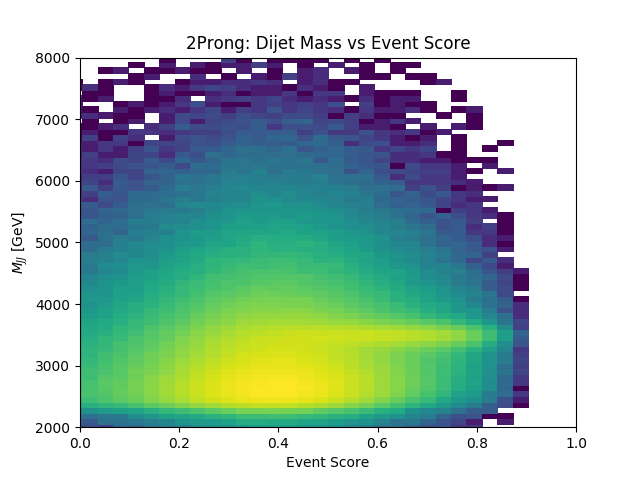
\includegraphics[width=0.5\textwidth]{imgs/ProcR_2Prong_Contaminated_10p0_2Prong_Contaminated_10p0_Weights_Event_ConstOnly_Avg_JJ_M_vs_Event_Score.png}
\caption{Description of the figure.  Reproduced from Ref.~\cite{Nachman:2020lpy}.}
\label{fig:m_v_s}
\end{figure}

\begin{figure}[h!]
	\begin{center}
		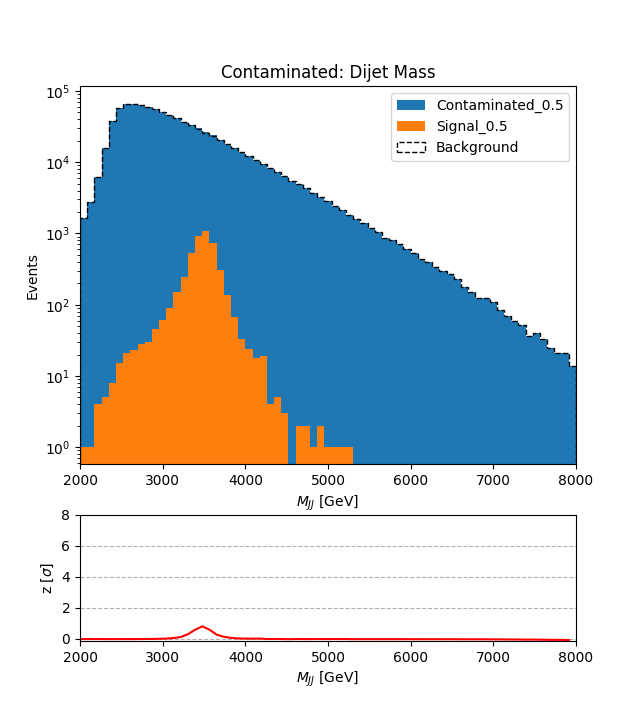
\includegraphics[width=0.49\textwidth]{imgs/2Prong_Contaminated_0p5_JJ_Mass_Multi.png}
		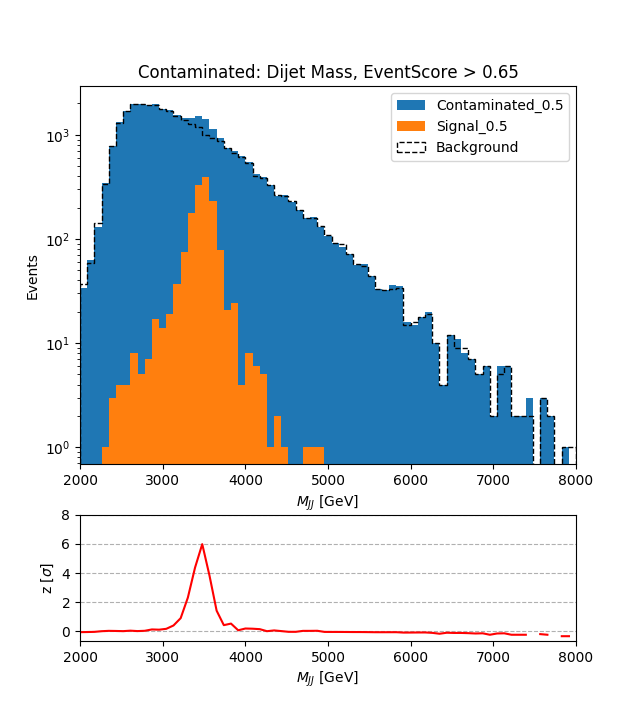
\includegraphics[width=0.49\textwidth]{imgs/2Prong_Contaminated_0p5_JJ_Mass_EventScore0p65_Multi.png}
	\end{center}
	\caption{Dijet mass distributions before (left) and after (right) a cut on the Event Score, at a signal contamination of 0.5\%}
	\label{fig:m_JJ}
\end{figure}

Our analysis on the Black Box datasets is performed by applying a cut on the Event Score at a value of 0.75, which is chosen to optimize the signal-to-background ratio, as well as restricting the pseudorapidity of the leading and sub-leading jets to less than 0.75 to ensure that central, high momentum-transfer events are being considered. Applying this method to Black Box 1, we arrive at the mass distributions of Figure {\ref{fig:bb1}}. Plotted here is the mass of the dijet combination for both the Black Box 1 dataset as well as the Background dataset, displayed as a dashed line. The important feature in this result is the shoulder present at around 4TeV, which corresponds to the present Z' signal at a mass of 3.8TeV. 

\begin{figure}[h!]
	\begin{center}
		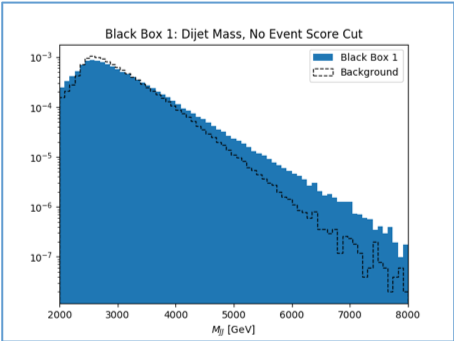
\includegraphics[width=0.49\textwidth]{imgs/BB1.png}
		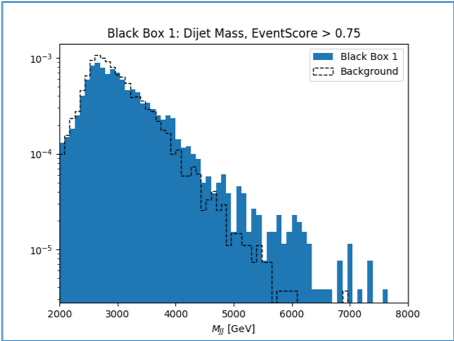
\includegraphics[width=0.49\textwidth]{imgs/BB1_Cut.png}
	\end{center}
	\caption{2-Prong dijet mass distributions before (left) and after (right) a cut on the Event Score, at a signal contamination of 0.5\%}
	\label{fig:bb1}
\end{figure}

In Black Box 2, our model shows no significant excesses. Furthermore, the behavior of the Event Score consistently affects the distributions of both Black Box 2 and the Background dataset. It is important to note that the model was trained independently on each dataset, and the resulting Event Scores are from entirely unique sets of network weights.

\begin{figure}[h!]
	\begin{center}
		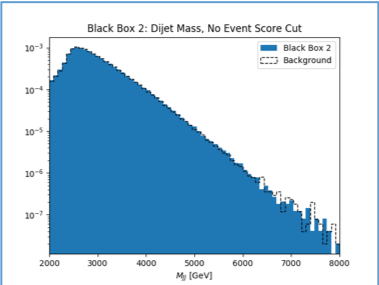
\includegraphics[width=0.49\textwidth]{imgs/BB2.png}
		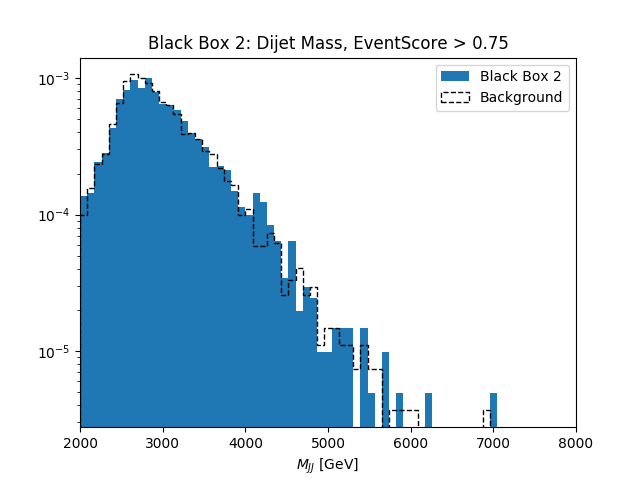
\includegraphics[width=0.49\textwidth]{imgs/BB2_Cut.png}
	\end{center}
	\caption{2-Prong dijet mass distributions before (left) and after (right) a cut on the Event Score, at a signal contamination of 0.5\%}
	\label{fig:bb2}
\end{figure}

Figure \ref{fig:bb3} shows our results for Black Box 3. Our model is specifically sensitive to boosted final states, and as a result, we are insensitive to the signal present in this Black Box. 

\begin{figure}[h!]
	\begin{center}
		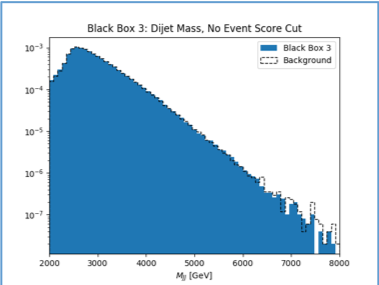
\includegraphics[width=0.49\textwidth]{imgs/BB3.png}
		\includegraphics[width=0.49\textwidth]{imgs/BB3_Cut.png}
	\end{center}
	\caption{2-Prong dijet mass distributions before (left) and after (right) a cut on the Event Score, at a signal contamination of 0.5\%}
	\label{fig:bb3}
\end{figure}


\subsection{Lessons Learned}
\label{sec:lessons}

%\noindent \textit{Please say anything that you learned from the experience in general, what you learned specifically from the results, what you improved after you learned about BB1, what you would change in the future, etc.}

This challenge presented a highly accessible avenue for development of our model. We are particularly surprised by the effect of our pre-processing method on the performance of the model, specifically by our choice of $k_{t}$-ordered sequencing, and find it to be a very interesting result which may have a number of applications in a wide range of analysis contexts. Overall, we view the VRNN as a model capable of identifying objects within a contaminated dataset as long as they can be characterized by sequential data. While we limited our scope in this study to be entirely unsupervised with absolutely no external information helping the model understand the elements of data that it is modeling, the accessibility of the VRNN's architecture, being both a RNN and a VAE, opens the possibility of accommodating more supervised training scenarios. We also restricted some of our development tracks in the interest of simplicity, but feel that a number of adjustments to the architecture, such as a dedicated adversarial mass de-correlation network, or an additional input layer representing high-level features, are worthwhile avenues of exploration.

%\subsection{Code Availability}
%\label{code:code}

%\noindent \textit{Please consider sharing a link to your code!  All of the sample links will be included in the paper so no need to add those.}

%%%%%%%%%%%%%%%%%%%%%%%%
\acknowledgments

This work was supported by the U.S.~Department of Energy, Office of Science under contract DE-AC02-05CH11231. 

\vspace{10mm}

\noindent \textit{For the references, please use names from Ref.~\cite{hepmllivingreview}.  If your paper is not there or is not updated, please submit a MR!}

\bibliographystyle{jhep}
\bibliography{HEPML}
\end{document}
